
\section*{Verkaveling}

Bij een verkaveling wordt een stuk land opgedeeld in verschillende kavels die elk een andere eigenaar kunnen hebben. Vroeger hadden de boeren kleine stukken land, die vaak door elkaar heen lagen. Een boer moest toen over het land van een andere boer lopen of rijden om naar zijn eigen kavels te gaan. Tengevolge van de schaalvergroting van de landbouw wordt tegenwoordig gewerkt met vierkante kavels, en streven boeren ernaar om te werken met zo groot mogelijke percelen: rechthoekige gebieden van aaneengesloten kavels.

Onderstaand voorbeeld toont een rechthoekig stuk land dat werd opgedeeld in $10 \times 10$ vierkante kavels. Drie percelen (witte rechthoeken) werden reeds door boeren in gebruik genomen. Zoek de oppervlakte van het grootst mogelijke perceel waarvan nog geen enkel kavel in gebruik werd genomen. In dit voorbeeld is dit een perceel dat bestaat uit 16 kavels, zoals aangegeven door de gestreepte rechthoek.

\begin{figure}[H]
  \center 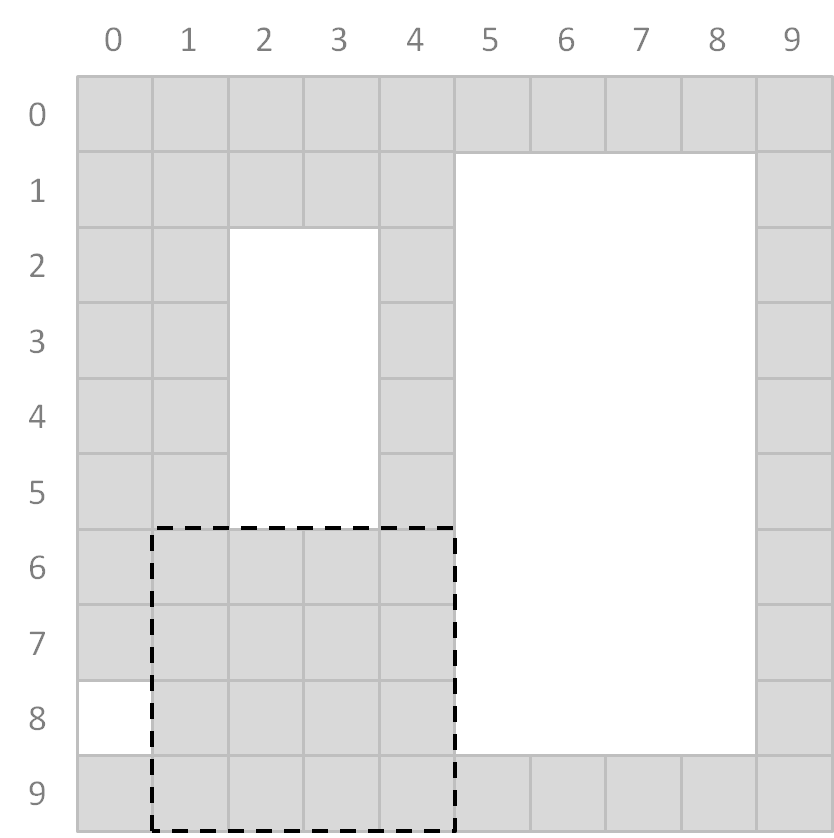
\includegraphics[scale=0.30]{verkaveling/verkaveling.png}
\end{figure}

\subsection*{Input}

De input voor deze opgave zal starten met een geheel getal dat het aantal
gevallen aanduid. Elk geval dat hierop volgt, bestaat uit meerdere regels. De
eerste bevat 2 strikt positieve gehele getallen, die de dimensies van de
verkaveling aanduiden. Het eerste getal stelt het aantal rijen voor, het tweede
het aantal kolommen. Na deze lijn volgt een lijn per rij van de matrix. Elk van
deze lijnen is even lang als het aantal kolommen van de matrix. Een \texttt{\#}
op zo'n lijn stelt een open plaats voor. Een \texttt{-} is dan weer een
ongebruikt kavel.

\subsubsection*{Voorbeeldinput}

\begin{verbatim}
2
8 12
############
############
############
############
############
############
############
############
8 12
############
############
############
#####--#####
#####--#####
############
############
############
\end{verbatim}

\subsection*{Output}

Per geval verwachten we de oppervlakte van het grootste perceel als geheel getal
op een lijn.

\subsubsection*{Voorbeeldoutput}

\begin{verbatim}
96
40
\end{verbatim}

